\documentclass[11pt,a4paper]{article}
\usepackage[margin=0.7in]{geometry}
\usepackage{tikz}
\usepackage{pgf-umlcd}
\usepackage{fontspec}
\usepackage{xcolor}
\usepackage{amsfonts}
\usepackage{amsmath}
\usepackage{listings}

% Configure emoji font for XeLaTeX (vector-based for better compatibility)
\newfontfamily\emojifont{Segoe UI Emoji}[
    Scale=1.0
]

% Create convenient emoji command
\newcommand{\emoji}[1]{{\emojifont #1}}

\usetikzlibrary{shapes,arrows,positioning,fit,backgrounds,decorations.pathmorphing,calc,shadows,matrix,chains,trees}

\title{PeiDocker Terminal GUI - Advanced Mode Design}
\author{Claude Code}
\date{\today}

\definecolor{primaryblue}{RGB}{51,122,183}
\definecolor{successgreen}{RGB}{92,184,92}
\definecolor{warningorange}{RGB}{240,173,78}
\definecolor{dangered}{RGB}{217,83,79}
\definecolor{lightgray}{RGB}{248,248,248}
\definecolor{darkgray}{RGB}{85,85,85}
\definecolor{infoblue}{RGB}{91,192,222}
\definecolor{purpleaccent}{RGB}{149,117,205}

\tikzset{
    % Advanced interface styles
    mainpanel/.style={
        rectangle, draw=primaryblue, thick, fill=lightgray!20,
        minimum width=16cm, minimum height=12cm,
        rounded corners=3pt
    },
    tabbar/.style={
        rectangle, draw=darkgray, fill=darkgray!20,
        minimum width=16cm, minimum height=1cm
    },
    tab/.style={
        rectangle, draw=darkgray, fill=lightgray,
        minimum width=2.5cm, minimum height=0.8cm,
        rounded corners=3pt
    },
    activetab/.style={
        rectangle, draw=primaryblue, thick, fill=white,
        minimum width=2.5cm, minimum height=0.8cm,
        rounded corners=3pt
    },
    formsection/.style={
        rectangle, draw=successgreen, fill=successgreen!10,
        text width=7cm, minimum height=3cm,
        rounded corners=3pt
    },
    configfield/.style={
        rectangle, draw=darkgray, fill=white,
        minimum width=4cm, minimum height=0.6cm,
        rounded corners=2pt
    },
    actionbtn/.style={
        rectangle, draw=primaryblue, thick, fill=primaryblue!30,
        minimum width=2.5cm, minimum height=0.7cm,
        rounded corners=3pt, font=\bfseries
    },
    sidepanel/.style={
        rectangle, draw=purpleaccent, fill=purpleaccent!10,
        text width=3.5cm, minimum height=8cm,
        rounded corners=3pt
    },
    yamlpanel/.style={
        rectangle, draw=darkgray, fill=darkgray!10,
        text width=7cm, minimum height=6cm,
        rounded corners=3pt, font=\ttfamily\footnotesize
    }
}

\lstset{
    basicstyle=\ttfamily\footnotesize,
    backgroundcolor=\color{lightgray!30},
    frame=single,
    breaklines=true,
    showstringspaces=false
}

\begin{document}

\maketitle

\section{Advanced Mode Interface Overview}

The Advanced Mode provides a comprehensive form-based interface that allows users to configure all aspects of their PeiDocker project. It features tabbed navigation, real-time YAML preview, template management, and direct editing capabilities.

\subsection{Main Interface Layout}

\begin{figure}[htbp]
\centering
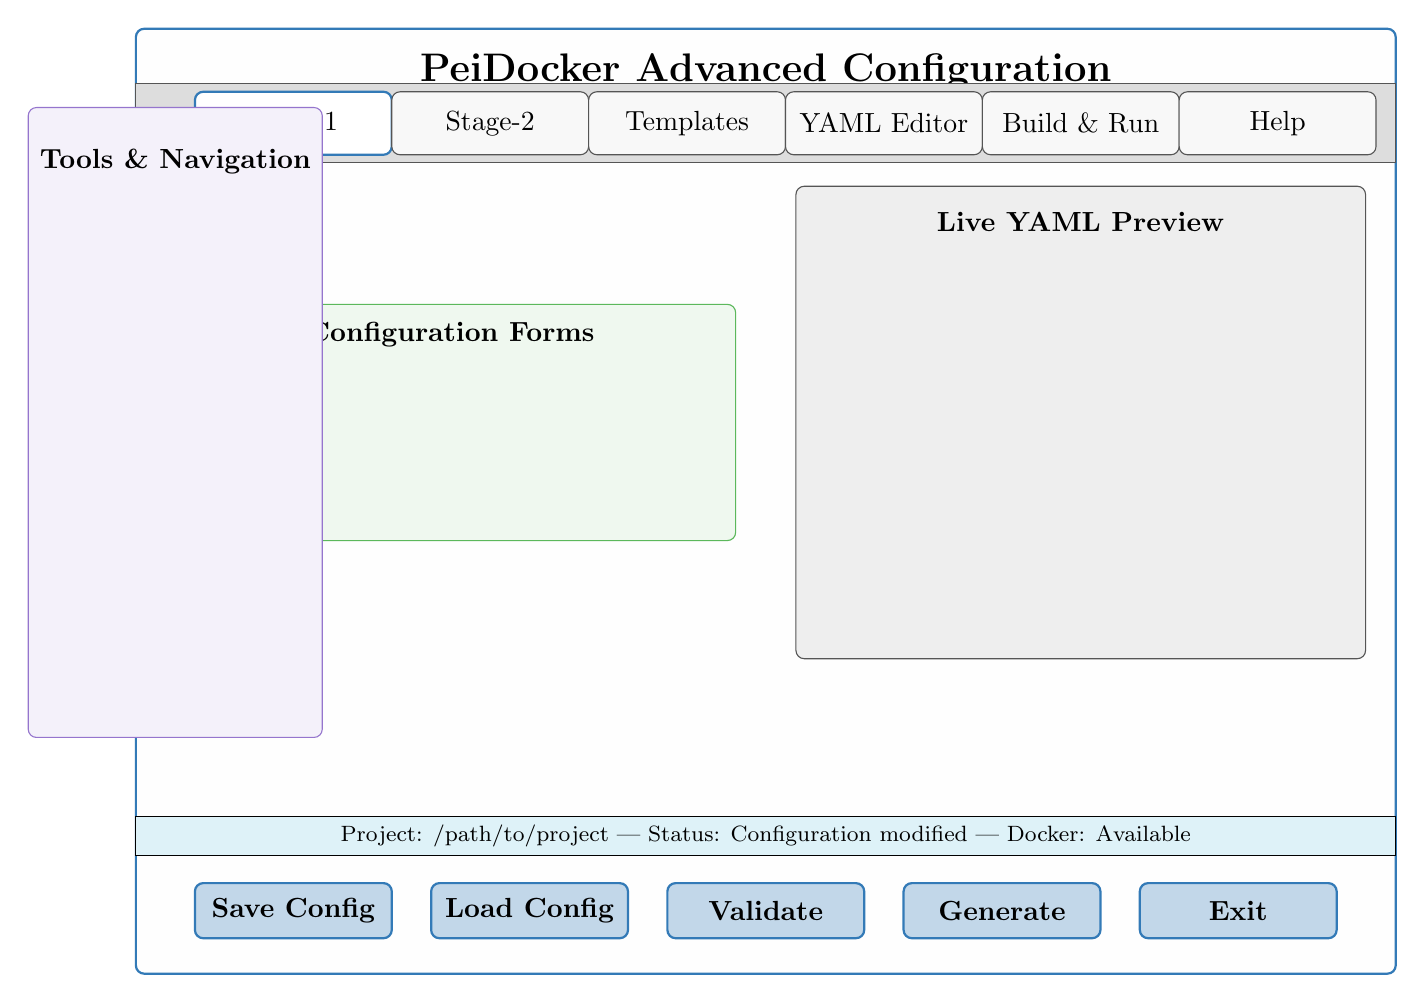
\begin{tikzpicture}

% Main window frame
\node[mainpanel] (main) at (0,0) {};

% Title bar
\node[anchor=north] at (0,5.8) {\Large\textbf{PeiDocker Advanced Configuration}};

% Tab bar
\node[tabbar] (tabs) at (0,4.8) {};

% Tabs
\node[activetab] at (-6.0,4.8) {Stage-1};
\node[tab] at (-3.5,4.8) {Stage-2};
\node[tab] at (-1.0,4.8) {Templates};
\node[tab] at (1.5,4.8) {YAML Editor};
\node[tab] at (4.0,4.8) {Build \& Run};
\node[tab] at (6.5,4.8) {Help};

% Main content area divided into sections
% Left panel - Configuration forms
\node[formsection] (forms) at (-4,1) {};
\node[anchor=north] at (-4,2.4) {\textbf{Configuration Forms}};

% Right panel - Live preview
\node[yamlpanel] (preview) at (4,1) {};
\node[anchor=north] at (4,3.8) {\textbf{Live YAML Preview}};

% Side panel - Navigation and tools
\node[sidepanel] (tools) at (-7.5,1) {};
\node[anchor=north] at (-7.5,4.6) {\textbf{Tools \& Navigation}};

% Status bar at bottom
\draw[fill=infoblue!20] (-8,-4.5) rectangle (8,-4);
\node[font=\footnotesize] at (0,-4.25) {Project: /path/to/project | Status: Configuration modified | Docker: Available};

% Navigation buttons
\node[actionbtn] at (-6,-5.2) {Save Config};
\node[actionbtn] at (-3,-5.2) {Load Config};
\node[actionbtn] at (0,-5.2) {Validate};
\node[actionbtn] at (3,-5.2) {Generate};
\node[actionbtn] at (6,-5.2) {Exit};

\end{tikzpicture}
\caption{Advanced Mode Main Interface Layout}
\end{figure}

\subsection{Stage-1 Configuration Tab}

\begin{figure}[htbp]
\centering
\begin{tikzpicture}

% Main panel
\draw[thick, fill=lightgray!20] (-8,-6) rectangle (8,6);
\node[anchor=north] at (0,5.7) {\Large\textbf{Stage-1 Configuration}};

% Left side - Form sections
\node[font=\large\bfseries] at (-5.5,4.8) {Basic Settings};

% Image settings
\draw[fill=successgreen!10] (-7.5,3.5) rectangle (-3.5,4.5);
\node[anchor=west, font=\bfseries] at (-7.3,4.2) {Image Configuration};
\node[anchor=west, font=\footnotesize] at (-7.3,4) {Base Image:};
\node[configfield] at (-5.5,4) {};
\node[anchor=west, font=\ttfamily] at (-6.8,4) {ubuntu:24.04};
\node[anchor=west, font=\footnotesize] at (-7.3,3.7) {Output Tag:};
\node[configfield] at (-5.5,3.7) {};
\node[anchor=west, font=\ttfamily] at (-6.8,3.7) {myproject:stage-1};

% SSH Configuration section
\draw[fill=infoblue!10] (-7.5,1.5) rectangle (-3.5,3.3);
\node[anchor=west, font=\bfseries] at (-7.3,3.1) {SSH Configuration};
\node[anchor=west, font=\footnotesize] at (-7.3,2.8) {Enable SSH:};
\draw[fill=successgreen] (-6.5,2.7) rectangle (-6.2,3);
\node[font=\tiny] at (-5.8,2.85) {\emoji{✓} Yes};

\node[anchor=west, font=\footnotesize] at (-7.3,2.5) {Container Port:};
\node[configfield, minimum width=1.5cm] at (-6,2.5) {};
\node[anchor=west, font=\ttfamily] at (-6.5,2.5) {22};

\node[anchor=west, font=\footnotesize] at (-7.3,2.2) {Host Port:};
\node[configfield, minimum width=1.5cm] at (-6,2.2) {};
\node[anchor=west, font=\ttfamily] at (-6.5,2.2) {2222};

% SSH Users subsection
\draw[fill=white] (-7.3,1.6) rectangle (-3.7,2.0);
\node[anchor=west, font=\tiny\bfseries] at (-7.2,1.9) {SSH Users};
\node[actionbtn, minimum width=1.5cm, minimum height=0.3cm] at (-4.2,1.8) {+ Add User};

% Users list
\draw[fill=lightgray!50] (-7.3,0.8) rectangle (-3.7,1.5);
\node[anchor=west, font=\tiny] at (-7.2,1.4) {\emoji{👤} me (UID: 1000) [password + pubkey]};
\node[anchor=west, font=\tiny] at (-7.2,1.2) {\emoji{👤} root (UID: 0) [password only]};
\node[anchor=west, font=\tiny] at (-7.2,1.0) {+ Click to edit user configuration};

% Proxy and APT section
\draw[fill=warningorange!10] (-7.5,-0.5) rectangle (-3.5,0.5);
\node[anchor=west, font=\bfseries] at (-7.3,0.3) {Network \& Packages};
\node[anchor=west, font=\footnotesize] at (-7.3,0) {Proxy:};
\draw (-6.5,-0.1) rectangle (-6.2,0.1);
\node[font=\tiny] at (-5.8,0) {Disabled};
\node[anchor=west, font=\footnotesize] at (-7.3,-0.3) {APT Mirror:};
\node[configfield, minimum width=1.5cm] at (-6,-0.3) {};
\node[anchor=west, font=\ttfamily] at (-6.5,-0.3) {tuna};

% Right side - Advanced settings
\node[font=\large\bfseries] at (1.5,4.8) {Advanced Settings};

% Environment variables
\draw[fill=purpleaccent!10] (-1,3.5) rectangle (4,4.5);
\node[anchor=west, font=\bfseries] at (-0.8,4.2) {Environment Variables};
\node[actionbtn, minimum width=1.5cm, minimum height=0.3cm] at (2.5,4.1) {+ Add Var};
\draw[fill=lightgray!50] (-0.8,3.6) rectangle (3.8,4);
\node[anchor=west, font=\tiny] at (-0.7,3.9) {DEBIAN\_FRONTEND=noninteractive};
\node[anchor=west, font=\tiny] at (-0.7,3.7) {LANG=en\_US.UTF-8};

% Ports mapping
\draw[fill=dangered!10] (-1,2.5) rectangle (4,3.3);
\node[anchor=west, font=\bfseries] at (-0.8,3.1) {Port Mapping};
\node[actionbtn, minimum width=1.5cm, minimum height=0.3cm] at (2.5,3) {+ Add Port};
\draw[fill=lightgray!50] (-0.8,2.6) rectangle (3.8,2.9);
\node[anchor=west, font=\tiny] at (-0.7,2.8) {2222:22 (SSH)};
\node[anchor=west, font=\tiny] at (-0.7,2.65) {8080:80 (HTTP)};

% Device and mounts
\draw[fill=successgreen!10] (-1,1.5) rectangle (4,2.3);
\node[anchor=west, font=\bfseries] at (-0.8,2.1) {Device \& Storage};
\node[anchor=west, font=\footnotesize] at (-0.8,1.9) {Device Type:};
\draw[fill=successgreen] (0.5,1.8) rectangle (0.8,2);
\node[font=\tiny] at (1.2,1.9) {\emoji{✓} CPU};
\draw (1.8,1.8) rectangle (2.1,2);
\node[font=\tiny] at (2.5,1.9) {GPU};

\node[anchor=west, font=\footnotesize] at (-0.8,1.7) {Mounts:};
\node[actionbtn, minimum width=1.5cm, minimum height=0.3cm] at (2.5,1.65) {+ Add Mount};

% Custom scripts
\draw[fill=infoblue!10] (-1,0.2) rectangle (4,1.3);
\node[anchor=west, font=\bfseries] at (-0.8,1.1) {Custom Scripts};

% Script types as tabs
\draw[fill=white] (-0.8,0.8) rectangle (0.2,1);
\node[font=\tiny] at (-0.3,0.9) {on\_build};
\draw (-0.2,0.8) rectangle (0.8,1);
\node[font=\tiny] at (0.3,0.9) {on\_first\_run};
\draw (0.8,0.8) rectangle (1.8,1);
\node[font=\tiny] at (1.3,0.9) {on\_every\_run};
\draw (1.8,0.8) rectangle (2.8,1);
\node[font=\tiny] at (2.3,0.9) {on\_user\_login};

\node[actionbtn, minimum width=1.5cm, minimum height=0.3cm] at (2.5,0.6) {+ Add Script};
\draw[fill=lightgray!50] (-0.8,0.3) rectangle (3.8,0.7);
\node[anchor=west, font=\tiny] at (-0.7,0.5) {stage-1/custom/install-dev-tools.sh};

% Far right - YAML Preview
\draw[fill=darkgray!10] (5,-5.5) rectangle (7.8,4.5);
\node[anchor=north, font=\bfseries] at (6.4,4.3) {Live Preview};
\node[anchor=north west, font=\ttfamily\tiny, text width=2.5cm, align=left] at (5.1,4) {
stage\_1:\\
\phantom{  }image:\\
\phantom{    }base: ubuntu:24.04\\
\phantom{    }output: myproject:stage-1\\
\phantom{  }ssh:\\
\phantom{    }enable: true\\
\phantom{    }port: 22\\
\phantom{    }host\_port: 2222\\
\phantom{    }users:\\
\phantom{      }me:\\
\phantom{        }password: '123456'\\
\phantom{        }pubkey\_file: ~/.ssh/id\_rsa.pub\\
\phantom{        }uid: 1000\\
\phantom{      }root:\\
\phantom{        }password: 'root'\\
\phantom{        }uid: 0\\
\phantom{  }proxy:\\
\phantom{    }enable\_globally: false\\
\phantom{  }apt:\\
\phantom{    }repo\_source: 'tuna'\\
\phantom{  }environment:\\
\phantom{    }- 'DEBIAN\_FRONTEND=...'\\
\phantom{  }ports:\\
\phantom{    }- '2222:22'\\
\phantom{    }- '8080:80'
};

% Bottom status and actions
\draw[fill=infoblue!20] (-8,-5.5) rectangle (4.8,-5);
\node[anchor=west, font=\footnotesize] at (-7.8,-5.25) {Modified: 3 changes pending | Validation: \emoji{✓} All fields valid};

\node[actionbtn, minimum width=1.8cm] at (-6.5,-6.2) {Reset Form};
\node[actionbtn, minimum width=1.8cm] at (-4.5,-6.2) {Load Template};
\node[actionbtn, minimum width=1.8cm] at (-2.5,-6.2) {Save Template};
\node[actionbtn, minimum width=1.8cm] at (-0.5,-6.2) {Validate};

\end{tikzpicture}
\caption{Stage-1 Configuration Tab Interface}
\end{figure}

\subsection{Stage-2 Configuration Tab}

\begin{figure}[htbp]
\centering
\begin{tikzpicture}

% Main panel
\draw[thick, fill=lightgray!20] (-8,-6) rectangle (8,6);
\node[anchor=north] at (0,5.7) {\Large\textbf{Stage-2 Configuration}};

% Inheritance notice
\draw[fill=infoblue!20] (-7.5,4.5) rectangle (7.5,5.5);
\node[anchor=north, font=\bfseries] at (0,5.3) {Stage-2 builds upon Stage-1 configuration};
\node[anchor=north, font=\footnotesize] at (0,5) {Settings here will override or extend Stage-1 where applicable};

% Left side - Storage configuration (main focus for Stage-2)
\node[font=\large\bfseries] at (-5.5,4) {Storage Configuration};

% Storage settings
\draw[fill=successgreen!10] (-7.5,2.5) rectangle (-3.5,4);
\node[anchor=west, font=\bfseries] at (-7.3,3.8) {Intelligent Storage};

% App storage
\node[anchor=west, font=\footnotesize] at (-7.3,3.5) {App Storage (/soft/app):};
\node[configfield, minimum width=2cm] at (-5.5,3.5) {};
\node[anchor=west, font=\ttfamily] at (-6.3,3.5) {auto-volume};

% Data storage
\node[anchor=west, font=\footnotesize] at (-7.3,3.2) {Data Storage (/soft/data):};
\node[configfield, minimum width=2cm] at (-5.5,3.2) {};
\node[anchor=west, font=\ttfamily] at (-6.3,3.2) {auto-volume};

% Workspace storage
\node[anchor=west, font=\footnotesize] at (-7.3,2.9) {Workspace (/soft/workspace):};
\node[configfield, minimum width=2cm] at (-5.5,2.9) {};
\node[anchor=west, font=\ttfamily] at (-6.3,2.9) {host};

% Host path for workspace (conditional)
\node[anchor=west, font=\footnotesize] at (-7.3,2.6) {Host Path:};
\node[configfield, minimum width=2.5cm] at (-5.2,2.6) {};
\node[anchor=west, font=\ttfamily] at (-6.5,2.6) {/home/user/workspace};

% Additional mounts
\draw[fill=purpleaccent!10] (-7.5,1) rectangle (-3.5,2.3);
\node[anchor=west, font=\bfseries] at (-7.3,2.1) {Additional Mounts};
\node[actionbtn, minimum width=1.5cm, minimum height=0.3cm] at (-4.5,1.9) {+ Add Mount};

% Mount list
\draw[fill=lightgray!50] (-7.3,1.1) rectangle (-3.7,1.8);
\node[anchor=west, font=\tiny] at (-7.2,1.7) {\emoji{📁} home\_me → /home/me (auto-volume)};
\node[anchor=west, font=\tiny] at (-7.2,1.5) {\emoji{📁} apt\_cache → /var/cache/apt (auto-volume)};
\node[anchor=west, font=\tiny] at (-7.2,1.3) {\emoji{📁} project\_data → /data (host: /host/data)};

% Center - Environment and overrides
\node[font=\large\bfseries] at (0,4) {Environment \& Overrides};

% Environment variables for stage-2
\draw[fill=warningorange!10] (-2.5,2.8) rectangle (2.5,3.8);
\node[anchor=west, font=\bfseries] at (-2.3,3.6) {Additional Environment Variables};
\node[actionbtn, minimum width=1.2cm, minimum height=0.3cm] at (1.5,3.5) {+ Add};
\draw[fill=lightgray!50] (-2.3,2.9) rectangle (2.3,3.3);
\node[anchor=west, font=\tiny] at (-2.2,3.2) {WORKSPACE\_PATH=/soft/workspace};
\node[anchor=west, font=\tiny] at (-2.2,3.0) {STAGE=production};

% Device override
\draw[fill=dangered!10] (-2.5,2) rectangle (2.5,2.6);
\node[anchor=west, font=\bfseries] at (-2.3,2.4) {Device Override};
\node[anchor=west, font=\footnotesize] at (-2.3,2.2) {Override Stage-1 device settings:};
\draw (-1,2.1) rectangle (-0.7,2.3);
\node[font=\tiny] at (-0.3,2.2) {No Override};

% Right side - Custom scripts for Stage-2
\node[font=\large\bfseries] at (5.5,4) {Stage-2 Custom Scripts};

\draw[fill=infoblue!10] (3.5,2.5) rectangle (7.5,3.8);
\node[anchor=west, font=\bfseries] at (3.7,3.6) {Application-Level Scripts};

% Script categories
\draw[fill=white] (3.7,3.2) rectangle (4.5,3.4);
\node[font=\tiny] at (4.1,3.3) {on\_build};
\draw[fill=successgreen] (4.5,3.2) rectangle (5.3,3.4);
\node[font=\tiny] at (4.9,3.3) {on\_first\_run};
\draw[fill=white] (5.3,3.2) rectangle (6.1,3.4);
\node[font=\tiny] at (5.7,3.3) {on\_every\_run};
\draw[fill=white] (6.1,3.2) rectangle (7,3.4);
\node[font=\tiny] at (6.55,3.3) {on\_user\_login};

\node[actionbtn, minimum width=1.2cm, minimum height=0.3cm] at (6.5,2.9) {+ Add Script};

% Script list for selected category
\draw[fill=lightgray!50] (3.7,2.6) rectangle (7.3,3.1);
\node[anchor=west, font=\tiny] at (3.8,3) {stage-2/custom/setup-workspace.sh --init};
\node[anchor=west, font=\tiny] at (3.8,2.8) {stage-2/custom/install-app-deps.sh};
\node[anchor=west, font=\tiny] at (3.8,2.65) {+ Click to add new on\_first\_run script};

% Entry point override
\draw[fill=purpleaccent!10] (3.5,1.5) rectangle (7.5,2.3);
\node[anchor=west, font=\bfseries] at (3.7,2.1) {Entry Point Override};
\node[anchor=west, font=\footnotesize] at (3.7,1.9) {Custom entry point (overrides Stage-1):};
\node[configfield, minimum width=3cm] at (5.8,1.7) {};
\node[anchor=west, font=\ttfamily] at (4.3,1.7) {stage-2/custom/app-start.sh};

% Bottom - Storage visualization diagram
\draw[fill=lightgray!30] (-7.5,-0.5) rectangle (7.5,0.8);
\node[anchor=north, font=\bfseries] at (0,0.7) {Storage Architecture Visualization};

% Storage flow diagram
% Soft links on left
\draw[fill=successgreen!20] (-6.5,-0.2) rectangle (-4.5,0.5);
\node[font=\tiny] at (-5.5,0.3) {/soft/app};
\node[font=\tiny] at (-5.5,0.1) {/soft/data};
\node[font=\tiny] at (-5.5,-0.1) {/soft/workspace};

% Arrows
\draw[->] (-4.3,0.3) -- (-3,0.3);
\draw[->] (-4.3,0.1) -- (-3,0.1);
\draw[->] (-4.3,-0.1) -- (-3,-0.1);

% Hard destinations
\draw[fill=infoblue!20] (-3,0.2) rectangle (-0.5,0.4);
\node[font=\tiny] at (-1.75,0.3) {/hard/volume/app};
\draw[fill=infoblue!20] (-3,0) rectangle (-0.5,0.2);
\node[font=\tiny] at (-1.75,0.1) {/hard/volume/data};
\draw[fill=warningorange!20] (-3,-0.2) rectangle (-0.5,0);
\node[font=\tiny] at (-1.75,-0.1) {/hard/volume/workspace};

% Alternative paths
\draw[->] (0,0.3) -- (1.5,0.3);
\draw[->] (0,0.1) -- (1.5,0.1);
\draw[->] (0,-0.1) -- (1.5,-0.1);

\draw[fill=lightgray!50] (1.7,0.2) rectangle (4,0.4);
\node[font=\tiny] at (2.85,0.3) {/hard/image/app (fallback)};
\draw[fill=lightgray!50] (1.7,0) rectangle (4,0.2);
\node[font=\tiny] at (2.85,0.1) {/hard/image/data (fallback)};
\draw[fill=successgreen!20] (1.7,-0.2) rectangle (4,0);
\node[font=\tiny] at (2.85,-0.1) {/host/user/workspace};

% Bottom actions
\draw[fill=infoblue!20] (-8,-5.5) rectangle (8,-5);
\node[anchor=west, font=\footnotesize] at (-7.8,-5.25) {Stage-2 Configuration | Storage: 3 volumes, 1 host mount | Scripts: 2 custom};

\node[actionbtn, minimum width=1.8cm] at (-6,-6.2) {Reset to Stage-1};
\node[actionbtn, minimum width=1.8cm] at (-3.5,-6.2) {Preview Storage};
\node[actionbtn, minimum width=1.8cm] at (-1,-6.2) {Test Mount Paths};
\node[actionbtn, minimum width=1.8cm] at (1.5,-6.2) {Validate Config};
\node[actionbtn, minimum width=1.8cm] at (4,-6.2) {Generate YAML};

\end{tikzpicture}
\caption{Stage-2 Configuration Tab Interface}
\end{figure}

\subsection{Templates Management Tab}

\begin{figure}[htbp]
\centering
\begin{tikzpicture}

% Main panel
\draw[thick, fill=lightgray!20] (-8,-6) rectangle (8,6);
\node[anchor=north] at (0,5.7) {\Large\textbf{Configuration Templates}};

% Left panel - Template browser
\draw[fill=successgreen!10] (-7.5,2) rectangle (-3,5.3);
\node[anchor=north, font=\bfseries] at (-5.25,5.1) {Available Templates};

% Template categories
\node[font=\footnotesize\bfseries] at (-5.25,4.7) {\emoji{📁} Built-in Templates};
\draw[fill=white] (-7.3,4.2) rectangle (-3.2,4.6);
\node[anchor=west, font=\tiny] at (-7.2,4.5) {\emoji{🐳} Basic Ubuntu Container};
\node[anchor=west, font=\tiny] at (-7.2,4.3) {\emoji{🤖} AI/ML Development (CUDA + Python)};
\draw[fill=white] (-7.3,3.8) rectangle (-3.2,4.2);
\node[anchor=west, font=\tiny] at (-7.2,4.1) {\emoji{🚀} ROS2 Robotics Environment};
\node[anchor=west, font=\tiny] at (-7.2,3.9) {\emoji{🌐} Web Development (Node.js + nginx)};

\node[font=\footnotesize\bfseries] at (-5.25,3.5) {\emoji{📁} User Templates};
\draw[fill=lightgray!50] (-7.3,2.8) rectangle (-3.2,3.4);
\node[anchor=west, font=\tiny] at (-7.2,3.3) {\emoji{💾} my-dev-environment (saved 2024-01-15)};
\node[anchor=west, font=\tiny] at (-7.2,3.1) {\emoji{💾} production-setup (saved 2024-01-10)};
\node[anchor=west, font=\tiny] at (-7.2,2.9) {\emoji{💾} testing-config (saved 2024-01-08)};

\node[actionbtn, minimum width=2cm, minimum height=0.4cm] at (-5.25,2.4) {+ New Template};
\node[actionbtn, minimum width=2cm, minimum height=0.4cm] at (-5.25,2.1) {Import Template};

% Center panel - Template details
\draw[fill=infoblue!10] (-2.5,2) rectangle (2.5,5.3);
\node[anchor=north, font=\bfseries] at (0,5.1) {Template Details};

% Selected template info
\node[font=\bfseries] at (0,4.7) {AI/ML Development Template};
\draw[fill=white] (-2.3,3.8) rectangle (2.3,4.5);
\node[anchor=north west, font=\tiny, text width=4.3cm, align=left] at (-2.2,4.4) {
\textbf{Description:} Complete environment for\\
machine learning development with CUDA\\
support, Jupyter, PyTorch, and TensorFlow.\\[0.5em]
\textbf{Base Image:} nvidia/cuda:12.1-devel-ubuntu22.04\\
\textbf{GPU Required:} Yes\\
\textbf{Estimated Size:} 8.5 GB
};

\node[font=\footnotesize\bfseries] at (0,3.6) {Included Components:};
\draw[fill=lightgray!50] (-2.3,2.8) rectangle (2.3,3.5);
\node[anchor=north west, font=\tiny, text width=4.3cm, align=left] at (-2.2,3.4) {
\emoji{✓} CUDA 12.1 development tools\\
\emoji{✓} Python 3.10 + pip + conda\\
\emoji{✓} Jupyter Lab + common ML libraries\\
\emoji{✓} SSH access with key authentication\\
\emoji{✓} VS Code server integration\\
\emoji{✓} TensorBoard and MLflow setup
};

\node[actionbtn, minimum width=2cm, minimum height=0.4cm] at (-1,2.4) {Apply Template};
\node[actionbtn, minimum width=2cm, minimum height=0.4cm] at (1,2.4) {Customize};

% Right panel - Template creation/editing
\draw[fill=purpleaccent!10] (3,2) rectangle (7.5,5.3);
\node[anchor=north, font=\bfseries] at (5.25,5.1) {Create/Edit Template};

\node[anchor=west, font=\footnotesize] at (3.2,4.8) {Template Name:};
\node[configfield, minimum width=3.5cm] at (5.5,4.8) {};
\node[anchor=west, font=\ttfamily] at (3.7,4.8) {my-custom-template};

\node[anchor=west, font=\footnotesize] at (3.2,4.5) {Description:};
\draw[fill=white] (3.2,4) rectangle (7.3,4.4);
\node[anchor=north west, font=\tiny, text width=3.8cm, align=left] at (3.3,4.35) {Custom development environment\\for my specific needs...};

\node[anchor=west, font=\footnotesize] at (3.2,3.7) {Base Configuration:};
\draw[fill=white] (3.2,3.2) rectangle (7.3,3.6);
\node[anchor=west, font=\tiny] at (3.3,3.5) {\emoji{◉} From current configuration};
\node[anchor=west, font=\tiny] at (3.3,3.3) {\emoji{○} From existing template};

\node[anchor=west, font=\footnotesize] at (3.2,2.9) {Include Components:};
\draw[fill=lightgray!50] (3.2,2.4) rectangle (7.3,2.8);
\node[anchor=west, font=\tiny] at (3.3,2.7) {\emoji{☑} SSH configuration \emoji{☑} Environment variables};
\node[anchor=west, font=\tiny] at (3.3,2.5) {\emoji{☑} Custom scripts \emoji{☐} Specific mount points};

\node[actionbtn, minimum width=1.5cm, minimum height=0.3cm] at (4.5,2.1) {Save Template};
\node[actionbtn, minimum width=1.2cm, minimum height=0.3cm] at (6.2,2.1) {Cancel};

% Bottom panel - Template operations
\draw[fill=warningorange!10] (-7.5,0.5) rectangle (7.5,1.8);
\node[anchor=north, font=\bfseries] at (0,1.6) {Template Operations};

% Import/Export section
\node[anchor=west, font=\footnotesize] at (-7.3,1.3) {Import from file:};
\node[configfield, minimum width=4cm] at (-4.5,1.3) {};
\node[anchor=west, font=\ttfamily] at (-6.2,1.3) {/path/to/template.yml};
\node[actionbtn, minimum width=1.2cm, minimum height=0.3cm] at (-2.3,1.3) {Browse};
\node[actionbtn, minimum width=1.2cm, minimum height=0.3cm] at (-1,1.3) {Import};

\node[anchor=west, font=\footnotesize] at (-7.3,0.9) {Export selected:};
\node[actionbtn, minimum width=1.5cm, minimum height=0.3cm] at (-5.5,0.9) {Export Template};
\node[actionbtn, minimum width=1.5cm, minimum height=0.3cm] at (-3.8,0.9) {Share Template};

% Sharing and collaboration
\node[anchor=west, font=\footnotesize] at (0.5,1.3) {Community Templates:};
\node[actionbtn, minimum width=1.5cm, minimum height=0.3cm] at (2.8,1.3) {Browse Online};
\node[actionbtn, minimum width=1.5cm, minimum height=0.3cm] at (4.5,1.3) {Submit Template};

\node[anchor=west, font=\footnotesize] at (0.5,0.9) {Backup \& Sync:};
\node[actionbtn, minimum width=1.2cm, minimum height=0.3cm] at (2.3,0.9) {Backup All};
\node[actionbtn, minimum width=1.2cm, minimum height=0.3cm] at (3.7,0.9) {Restore};

% Bottom status
\draw[fill=infoblue!20] (-8,-5.5) rectangle (8,-5);
\node[anchor=west, font=\footnotesize] at (-7.8,-5.25) {Templates: 15 built-in, 3 user-created | Selected: AI/ML Development | Status: Ready to apply};

\node[actionbtn, minimum width=1.8cm] at (-5.5,-6.2) {Apply \& Configure};
\node[actionbtn, minimum width=1.8cm] at (-3,-6.2) {Merge with Current};
\node[actionbtn, minimum width=1.8cm] at (-0.5,-6.2) {Preview Changes};
\node[actionbtn, minimum width=1.8cm] at (2,-6.2) {Reset to Template};

\end{tikzpicture}
\caption{Templates Management Tab Interface}
\end{figure}

\subsection{YAML Editor Tab}

\begin{figure}[htbp]
\centering
\begin{tikzpicture}

% Main panel
\draw[thick, fill=lightgray!20] (-8,-6) rectangle (8,6);
\node[anchor=north] at (0,5.7) {\Large\textbf{Direct YAML Editor}};

% Left panel - YAML editor
\draw[fill=darkgray!10] (-7.5,0) rectangle (-0.5,5.3);
\node[anchor=north, font=\bfseries] at (-4,5.1) {Configuration Editor};

% Editor toolbar
\draw[fill=darkgray!30] (-7.5,4.7) rectangle (-0.5,5.1);
\node[actionbtn, minimum width=1cm, minimum height=0.3cm] at (-6.8,4.9) {\emoji{📁} Open};
\node[actionbtn, minimum width=1cm, minimum height=0.3cm] at (-5.6,4.9) {\emoji{💾} Save};
\node[actionbtn, minimum width=1cm, minimum height=0.3cm] at (-4.4,4.9) {\emoji{↶} Undo};
\node[actionbtn, minimum width=1cm, minimum height=0.3cm] at (-3.2,4.9) {\emoji{↷} Redo};
\node[actionbtn, minimum width=1cm, minimum height=0.3cm] at (-2,4.9) {\emoji{🔍} Find};
\node[actionbtn, minimum width=1cm, minimum height=0.3cm] at (-0.8,4.9) {\emoji{✓} Format};

% YAML content area with syntax highlighting
\draw[fill=white] (-7.3,0.2) rectangle (-0.7,4.6);
\node[anchor=north west, font=\ttfamily\tiny, text width=6.3cm, align=left] at (-7.2,4.5) {
\textcolor{purple}{stage\_1:}\\
\phantom{  }\textcolor{purple}{image:}\\
\phantom{    }\textcolor{blue}{base:} ubuntu:24.04\\
\phantom{    }\textcolor{blue}{output:} myproject:stage-1\\
\phantom{  }\textcolor{purple}{ssh:}\\
\phantom{    }\textcolor{blue}{enable:} \textcolor{red}{true}\\
\phantom{    }\textcolor{blue}{port:} \textcolor{orange}{22}\\
\phantom{    }\textcolor{blue}{host\_port:} \textcolor{orange}{2222}\\
\phantom{    }\textcolor{purple}{users:}\\
\phantom{      }\textcolor{blue}{me:}\\
\phantom{        }\textcolor{blue}{password:} \textcolor{successgreen}{'123456'}\\
\phantom{        }\textcolor{blue}{pubkey\_file:} \textcolor{successgreen}{'~/.ssh/id\_rsa.pub'}\\
\phantom{        }\textcolor{blue}{uid:} \textcolor{orange}{1000}\\
\phantom{  }\textcolor{purple}{proxy:}\\
\phantom{    }\textcolor{blue}{address:} host.docker.internal\\
\phantom{    }\textcolor{blue}{port:} \textcolor{orange}{7890}\\
\phantom{    }\textcolor{blue}{enable\_globally:} \textcolor{red}{false}\\
\phantom{  }\textcolor{purple}{environment:}\\
\phantom{    }\textcolor{blue}{-} \textcolor{successgreen}{'DEBIAN\_FRONTEND=noninteractive'}\\
\phantom{    }\textcolor{blue}{-} \textcolor{successgreen}{'LANG=en\_US.UTF-8'}\\
\phantom{  }\textcolor{purple}{ports:}\\
\phantom{    }\textcolor{blue}{-} \textcolor{successgreen}{'2222:22'}\\
\phantom{    }\textcolor{blue}{-} \textcolor{successgreen}{'8080:80'}\\
\phantom{  }\textcolor{purple}{custom:}\\
\phantom{    }\textcolor{purple}{on\_build:}\\
\phantom{      }\textcolor{blue}{-} \textcolor{successgreen}{'stage-1/custom/install-dev.sh'}
};

% Line numbers
\node[anchor=north west, font=\ttfamily\tiny, color=darkgray, text width=1cm, align=left] at (-7.5,4.5) {
1\\2\\3\\4\\5\\6\\7\\8\\9\\10\\11\\12\\13\\14\\15\\16\\17\\18\\19\\20\\21\\22\\23\\24\\25
};

% Right panel - Editor features
\draw[fill=infoblue!10] (0,2.5) rectangle (7.5,5.3);
\node[anchor=north, font=\bfseries] at (3.75,5.1) {Editor Features \& Validation};

% Validation section
\node[font=\bfseries] at (3.75,4.7) {Real-time Validation};
\draw[fill=successgreen!20] (0.2,4.2) rectangle (7.3,4.5);
\node[anchor=west, font=\tiny] at (0.3,4.4) {\emoji{✓} YAML syntax valid};
\node[anchor=west, font=\tiny] at (0.3,4.25) {\emoji{✓} All required fields present};

\draw[fill=warningorange!20] (0.2,3.9) rectangle (7.3,4.1);
\node[anchor=west, font=\tiny] at (0.3,4) {\emoji{⚠} Line 12: Port 8080 may conflict with existing services};

% Schema validation
\node[font=\bfseries] at (3.75,3.6) {Schema Validation};
\draw[fill=lightgray!50] (0.2,3.1) rectangle (7.3,3.5);
\node[anchor=west, font=\tiny] at (0.3,3.4) {Schema: PeiDocker v2.1 (latest)};
\node[anchor=west, font=\tiny] at (0.3,3.3) {Compliance: 98\% (2 minor warnings)};
\node[anchor=west, font=\tiny] at (0.3,3.2) {Environment variables: 2 defined, 0 conflicts};
\node[anchor=west, font=\tiny] at (0.3,3.1) {Port mappings: 2 defined, 1 potential conflict};

\node[actionbtn, minimum width=1.5cm, minimum height=0.3cm] at (6.2,2.8) {Validate Schema};

% Bottom right - Autocomplete and help
\draw[fill=purpleaccent!10] (0,0) rectangle (7.5,2.3);
\node[anchor=north, font=\bfseries] at (3.75,2.1) {Smart Editing Features};

% Autocomplete
\node[anchor=west, font=\footnotesize] at (0.2,1.8) {Autocomplete \& IntelliSense:};
\draw[fill=white] (0.2,1.4) rectangle (7.3,1.7);
\node[anchor=west, font=\tiny] at (0.3,1.65) {• Field suggestions based on context};
\node[anchor=west, font=\tiny] at (0.3,1.55) {• Value validation for enums and types};
\node[anchor=west, font=\tiny] at (0.3,1.45) {• Template snippet insertion (Ctrl+Space)};

% Error highlighting
\node[anchor=west, font=\footnotesize] at (0.2,1.2) {Error Highlighting:};
\draw[fill=white] (0.2,0.8) rectangle (7.3,1.1);
\node[anchor=west, font=\tiny] at (0.3,1.05) {• Syntax errors highlighted in red};
\node[anchor=west, font=\tiny] at (0.3,0.95) {• Type mismatches shown with squiggly underlines};
\node[anchor=west, font=\tiny] at (0.3,0.85) {• Hover for detailed error messages};

% Quick fixes
\node[anchor=west, font=\footnotesize] at (0.2,0.6) {Quick Fixes:};
\draw[fill=white] (0.2,0.1) rectangle (7.3,0.5);
\node[anchor=west, font=\tiny] at (0.3,0.45) {• Auto-fix common YAML formatting issues};
\node[anchor=west, font=\tiny] at (0.3,0.35) {• Convert between different volume types};
\node[anchor=west, font=\tiny] at (0.3,0.25) {• Generate missing required fields};
\node[anchor=west, font=\tiny] at (0.3,0.15) {• Standardize environment variable formats};

% Bottom - File operations and tools
\draw[fill=infoblue!20] (-8,-5.5) rectangle (8,-5);
\node[anchor=west, font=\footnotesize] at (-7.8,-5.25) {File: user\_config.yml | Modified: Yes | Lines: 156 | Cursor: 25:12 | Encoding: UTF-8};

\node[actionbtn, minimum width=1.5cm] at (-6.5,-6.2) {Load File};
\node[actionbtn, minimum width=1.5cm] at (-4.8,-6.2) {Save File};
\node[actionbtn, minimum width=1.5cm] at (-3.1,-6.2) {Export};
\node[actionbtn, minimum width=1.5cm] at (-1.4,-6.2) {Format};
\node[actionbtn, minimum width=1.5cm] at (0.3,-6.2) {Validate};
\node[actionbtn, minimum width=1.5cm] at (2,-6.2) {Preview};
\node[actionbtn, minimum width=1.5cm] at (3.7,-6.2) {Generate};

\end{tikzpicture}
\caption{YAML Editor Tab Interface}
\end{figure}

\subsection{Build \& Run Tab}

\begin{figure}[htbp]
\centering
\begin{tikzpicture}

% Main panel
\draw[thick, fill=lightgray!20] (-8,-6) rectangle (8,6);
\node[anchor=north] at (0,5.7) {\Large\textbf{Build \& Run Management}};

% Left panel - Build process
\draw[fill=successgreen!10] (-7.5,1.5) rectangle (-2.5,5.3);
\node[anchor=north, font=\bfseries] at (-5,5.1) {Build Process};

% Build stages
\node[font=\bfseries] at (-5,4.7) {Build Stages};

% Stage 1 build
\draw[fill=infoblue!20] (-7.3,4) rectangle (-2.7,4.5);
\node[anchor=west, font=\footnotesize] at (-7.2,4.3) {Stage-1 Build};
\node[actionbtn, minimum width=1.2cm, minimum height=0.3cm] at (-3.5,4.25) {\emoji{▶} Build};
\draw[fill=successgreen] (-7.2,4.05) rectangle (-6.9,4.25);
\node[font=\tiny] at (-6.5,4.15) {\emoji{✓} Ready};

% Stage 2 build
\draw[fill=purpleaccent!20] (-7.3,3.5) rectangle (-2.7,4);
\node[anchor=west, font=\footnotesize] at (-7.2,3.8) {Stage-2 Build};
\node[actionbtn, minimum width=1.2cm, minimum height=0.3cm] at (-3.5,3.75) {\emoji{▶} Build};
\draw[fill=warningorange] (-7.2,3.55) rectangle (-6.9,3.75);
\node[font=\tiny] at (-6.5,3.65) {\emoji{⚠} Pending};

% Build options
\node[font=\bfseries] at (-5,3.2) {Build Options};
\draw[fill=white] (-7.3,2.7) rectangle (-2.7,3.1);
\node[anchor=west, font=\tiny] at (-7.2,3) {\emoji{☑} No cache (--no-cache)};
\node[anchor=west, font=\tiny] at (-7.2,2.85) {\emoji{☐} Parallel build (--parallel)};
\node[anchor=west, font=\tiny] at (-7.2,2.7) {\emoji{☑} Verbose output (--verbose)};

% Quick actions
\node[actionbtn, minimum width=2cm, minimum height=0.4cm] at (-5,2.3) {\emoji{🔨} Build All};
\node[actionbtn, minimum width=2cm, minimum height=0.4cm] at (-5,1.9) {\emoji{🧹} Clean \& Rebuild};

% Center panel - Runtime management
\draw[fill=infoblue!10] (-2,1.5) rectangle (3,5.3);
\node[anchor=north, font=\bfseries] at (0.5,5.1) {Container Runtime};

% Container status
\node[font=\bfseries] at (0.5,4.7) {Container Status};
\draw[fill=successgreen!20] (-1.8,4.2) rectangle (2.8,4.5);
\node[anchor=west, font=\tiny] at (-1.7,4.4) {\emoji{📦} myproject-stage-2: Running (PID: 12345)};
\node[anchor=west, font=\tiny] at (-1.7,4.25) {\emoji{🌐} SSH: localhost:2222 | HTTP: localhost:8080};

% Container actions
\node[font=\bfseries] at (0.5,3.9) {Container Actions};
\node[actionbtn, minimum width=1.5cm, minimum height=0.3cm] at (-0.5,3.6) {\emoji{▶} Start};
\node[actionbtn, minimum width=1.5cm, minimum height=0.3cm] at (1.5,3.6) {\emoji{⏹} Stop};
\node[actionbtn, minimum width=1.5cm, minimum height=0.3cm] at (-0.5,3.2) {\emoji{🔄} Restart};
\node[actionbtn, minimum width=1.5cm, minimum height=0.3cm] at (1.5,3.2) {\emoji{🗑} Remove};

% Quick access
\node[font=\bfseries] at (0.5,2.8) {Quick Access};
\node[actionbtn, minimum width=1.8cm, minimum height=0.3cm] at (0.5,2.5) {\emoji{🖥} SSH Connect};
\node[actionbtn, minimum width=1.8cm, minimum height=0.3cm] at (0.5,2.2) {\emoji{📁} Open Workspace};
\node[actionbtn, minimum width=1.8cm, minimum height=0.3cm] at (0.5,1.9) {\emoji{📊} View Logs};

% Right panel - Build monitoring
\draw[fill=warningorange!10] (3.5,1.5) rectangle (7.5,5.3);
\node[anchor=north, font=\bfseries] at (5.5,5.1) {Build Monitor};

% Real-time build output
\node[font=\bfseries] at (5.5,4.7) {Live Build Output};
\draw[fill=black] (3.7,3.5) rectangle (7.3,4.5);
\node[anchor=north west, font=\ttfamily\tiny, color=white, text width=3.3cm, align=left] at (3.8,4.4) {
\lbrack INFO\rbrack Building stage-1 image...\\
\lbrack INFO\rbrack Step 1/15: FROM ubuntu:24.04\\
\lbrack INFO\rbrack Step 2/15: RUN apt-get update\\
\lbrack INFO\rbrack \emoji{✓} Successfully installed packages\\
\lbrack INFO\rbrack Step 3/15: Setting up SSH server\\
\lbrack INFO\rbrack \emoji{⚠} Warning: Using default SSH keys\\
\lbrack INFO\rbrack Step 4/15: Configuring users...\\
\lbrack INFO\rbrack Current step: Installing custom scripts\\
\lbrack PROGRESS\rbrack 8/15 steps completed (53\%)
};

% Build statistics
\node[font=\bfseries] at (5.5,3.2) {Build Statistics};
\draw[fill=lightgray!50] (3.7,2.5) rectangle (7.3,3.1);
\node[anchor=west, font=\tiny] at (3.8,3) {\emoji{⏱} Elapsed Time: 4m 32s};
\node[anchor=west, font=\tiny] at (3.8,2.9) {\emoji{📦} Image Size: 2.1 GB (estimated)};
\node[anchor=west, font=\tiny] at (3.8,2.8) {\emoji{🔧} Build Cache: 1.2 GB saved};
\node[anchor=west, font=\tiny] at (3.8,2.7) {\emoji{📊} Progress: 53\% complete};
\node[anchor=west, font=\tiny] at (3.8,2.6) {\emoji{⏱} ETA: 3m 45s remaining};

% Error/warning summary
\node[font=\bfseries] at (5.5,2.3) {Issues Summary};
\draw[fill=white] (3.7,1.6) rectangle (7.3,2.2);
\node[anchor=west, font=\tiny] at (3.8,2.1) {\emoji{❌} Errors: 0};
\node[anchor=west, font=\tiny] at (3.8,2) {\emoji{⚠} Warnings: 2 (SSH key security, port conflicts)};
\node[anchor=west, font=\tiny] at (3.8,1.9) {\emoji{ℹ} Info: 15 (package installations, user setup)};
\node[anchor=west, font=\tiny] at (3.8,1.8) {\emoji{📋} Last issue: Warning about default SSH configuration};
\node[anchor=west, font=\tiny] at (3.8,1.7) {\emoji{🔍} Click any issue for details and solutions};

% Bottom panel - Docker integration
\draw[fill=purpleaccent!10] (-7.5,0) rectangle (7.5,1.3);
\node[anchor=north, font=\bfseries] at (0,1.1) {Docker Integration \& Advanced Tools};

% Docker status
\node[anchor=west, font=\footnotesize] at (-7.3,0.8) {Docker Status:};
\draw[fill=successgreen] (-5.8,0.7) rectangle (-5.5,0.9);
\node[font=\tiny] at (-5,0.8) {\emoji{✓} Docker Engine: 24.0.6 (running)};
\node[anchor=west, font=\tiny] at (-3.5,0.8) {Docker Compose: 2.21.0 | BuildKit: enabled};

% Image management
\node[anchor=west, font=\footnotesize] at (-7.3,0.5) {Image Management:};
\node[actionbtn, minimum width=1.2cm, minimum height=0.25cm] at (-5.5,0.45) {\emoji{📋} List Images};
\node[actionbtn, minimum width=1.2cm, minimum height=0.25cm] at (-4,0.45) {\emoji{🧹} Cleanup};
\node[actionbtn, minimum width=1.2cm, minimum height=0.25cm] at (-2.5,0.45) {\emoji{📤} Export};

% Advanced tools
\node[anchor=west, font=\footnotesize] at (0.5,0.8) {Advanced Tools:};
\node[actionbtn, minimum width=1.2cm, minimum height=0.25cm] at (2.5,0.8) {\emoji{🔍} Inspect};
\node[actionbtn, minimum width=1.2cm, minimum height=0.25cm] at (4,0.8) {\emoji{📊} Stats};
\node[actionbtn, minimum width=1.2cm, minimum height=0.25cm] at (5.5,0.8) {\emoji{🖥} Shell};

\node[anchor=west, font=\footnotesize] at (0.5,0.5) {Registry Integration:};
\node[actionbtn, minimum width=1.2cm, minimum height=0.25cm] at (2.5,0.45) {\emoji{📤} Push};
\node[actionbtn, minimum width=1.2cm, minimum height=0.25cm] at (4,0.45) {\emoji{📥} Pull};
\node[actionbtn, minimum width=1.2cm, minimum height=0.25cm] at (5.5,0.45) {\emoji{🏷} Tag};

% Bottom status bar
\draw[fill=infoblue!20] (-8,-5.5) rectangle (8,-5);
\node[anchor=west, font=\footnotesize] at (-7.8,-5.25) {Build Status: Stage-1 complete, Stage-2 in progress | Container: Running | Last build: 2 minutes ago};

\node[actionbtn, minimum width=1.5cm] at (-6,-6.2) {\emoji{⏹} Stop Build};
\node[actionbtn, minimum width=1.5cm] at (-4.2,-6.2) {\emoji{🔄} Rebuild All};
\node[actionbtn, minimum width=1.5cm] at (-2.4,-6.2) {\emoji{📋} Build Logs};
\node[actionbtn, minimum width=1.5cm] at (-0.6,-6.2) {\emoji{🖥} Container Shell};
\node[actionbtn, minimum width=1.5cm] at (1.2,-6.2) {\emoji{🌐} Open Ports};
\node[actionbtn, minimum width=1.5cm] at (3,-6.2) {\emoji{📊} Monitor};

\end{tikzpicture}
\caption{Build \& Run Management Tab Interface}
\end{figure}

\section{Advanced Mode Interaction Patterns}

\subsection{Form-Based Configuration Principles}

The Advanced Mode follows several key design principles:

\begin{itemize}
    \item \textbf{Non-linear Navigation}: Users can jump between any configuration section
    \item \textbf{Real-time Validation}: Immediate feedback on field values and relationships
    \item \textbf{Live Preview}: YAML configuration updates as users modify forms
    \item \textbf{Template Integration}: Built-in and user-defined templates for quick setup
    \item \textbf{Direct YAML Editing}: Power users can edit configuration directly
    \item \textbf{Build Integration}: Seamless transition from configuration to deployment
\end{itemize}

\subsection{State Management}

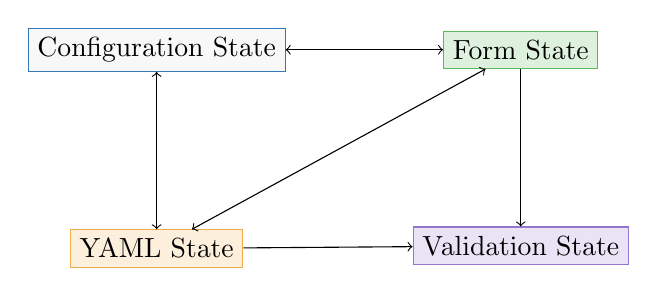
\begin{tikzpicture}[node distance=2cm]

\node[rectangle, draw=primaryblue, fill=lightgray] (config_state) {Configuration State};
\node[rectangle, draw=successgreen, fill=successgreen!20, right=of config_state] (form_state) {Form State};
\node[rectangle, draw=warningorange, fill=warningorange!20, below=of config_state] (yaml_state) {YAML State};
\node[rectangle, draw=purpleaccent, fill=purpleaccent!20, below=of form_state] (validation_state) {Validation State};

\draw[<->] (config_state) -- (form_state);
\draw[<->] (config_state) -- (yaml_state);
\draw[->] (form_state) -- (validation_state);
\draw[->] (yaml_state) -- (validation_state);
\draw[<->] (yaml_state) -- (form_state);

\end{tikzpicture}

\subsection{Error Handling and Recovery}

The Advanced Mode provides comprehensive error handling:

\begin{itemize}
    \item \textbf{Field-level Validation}: Real-time validation with inline error messages
    \item \textbf{Cross-field Dependencies}: Validation of relationships between configuration sections
    \item \textbf{Schema Compliance}: Ensure generated YAML matches PeiDocker schema
    \item \textbf{Recovery Suggestions}: Actionable suggestions for fixing configuration issues
    \item \textbf{Auto-save}: Prevent data loss with automatic configuration saving
\end{itemize}

\end{document}